\section{Перцептрон}

В работе будет использоваться нейронная сеть, основанная на модели перцептрона. Данная модель выбрана по нескольким критериям: во-первых она достаточно проста в изучении, во-вторых данная модель подходит для решения задачи, в-третьих модель перцептрона имеет простую реализацию на языке Python.  
Перцептроны передают информацию от входа к выходу. Нейронные сети часто описываются в виде слоев нейронов, где каждый слой состоит из входных, скрытых или выходных клеток. Клетки одного слоя не связаны между собой, а соседние слои обычно полностью связаны (Рис. 1.1). 

\begin{figure}[h]
  \centering
  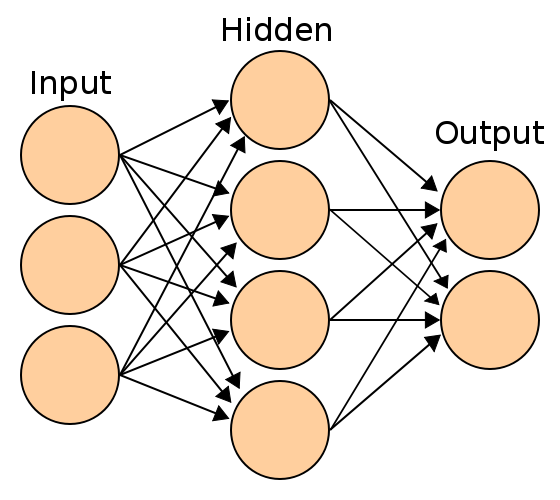
\includegraphics[width=0.5\linewidth]{./img/neural-network}
  \caption{Нейронная сеть}
  \label{fig:mpr}
\end{figure} 

Самая простая нейронная сеть имеет две входных клетки и одну выходную, и может использоваться в качестве модели логических вентилей. Нейронная сеть прямого распространения обычно обучается по методу обратного распространения ошибки, в котором модель получает множества входных и выходных данных. Этот процесс называется обучением с учителем, и он отличается от обучения без учителя тем, что во втором случае множество выходных данных сеть составляет самостоятельно.

Модель перцептрона была предложена и популяризована Ф. Розенблаттом. В начале 1960-х. Розенблатт верил в свою модель, и надеялся, что с помощью перцептрона человечество продвинется в создании искусственного интеллекта. В те времена была большая надежда на эту модель. Но в 1969 году Марвин Минский и Сеймур Паперт выпустили книгу, в которой рассматривали вычислительные способности перцептронов – то, чему могут учиться и чему не могут учиться перцептроны. И в том числе показывали некоторые ограничения модели. И, как часто это бывает, завышенные ожидания сменились чрезмерным разочарованием. В итоге критика, которая заключалась в доказательстве ограничения такой модели как перцептрон была обобщена на все нейросетевые модели и привела к застою в исследовании данной области на долгие годы.

Обучение перцептрона заключается в том, что ему «показывают» примеры и правильные ответы для этих примеров. Сперва веса перцептрона инициализируются случайно. И поэтому перцептрон, когда ему на вход поступает какой-нибудь пример, дает случайный ответ. Но мы бы хотели, чтобы перцептрон от случайных весов перешел к «осмысленным» весам, а значит, и к осмысленным ответам. 

Перцептрон (линейный нейрон) – это оператор вида: 


\begin{displaymath}
 f( \boldsymbol{x}, \boldsymbol{w}, b)  = 
  \begin{cases}
    1, \text{ если } \mathlarger{ \sum_{i=1}^{n} \boldsymbol{w_i} \boldsymbol{x_i} + b > 0} \\
    0 \text{иначе}
  \end{cases}
  \eqno(1)
\end{displaymath} \\

Где $f( \boldsymbol{x}, \boldsymbol{w}, b)$ - активационная функция; 

$ \mathlarger{ \sum_{i=1}^{n} \boldsymbol{w_i} \boldsymbol{x_i} + b > 0} $ - сумматорная функция; 

$\boldsymbol{x}$ - вектор входных активаций; 

$\boldsymbol{w}$ - вектор весов;

$b$ - смещение;


\begin{figure}[h]
  \centering
  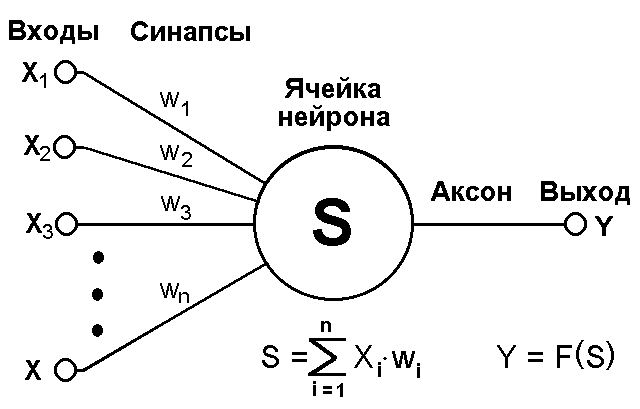
\includegraphics[width=0.5\linewidth]{./img/perceptron}
  \caption{Нейрон}
  \label{fig:mpr}
\end{figure} 

Модель перцептрона принимает несколько вещественных входных данных и дает один двоичный выход. В модели перцептрона каждый вход $x_i$ имеет вес, $w_i$ связанный с ним.
Веса указывают на важность ввода в процессе принятия решений. Выход модели определяется сумматорной функцией, если сумматорная функция больше нуля, то выход будет равен 1, иначе выход будет равен 0. Другими словами, модель будет срабатывать, если взвешенная сумма больше порога. 
Такой линейный нейрон способ решать лишь ряд простых задач, для которых хватает линейной функции, например, предсказание стоимости квартиры от ее площади или роста собаки от ее веса. 

К неприятным особенностям линейного нейрона можно отнести то, что небольшое изменение весов или смещений любого отдельного персептрона в сети может иногда приводить к тому, что выход этого персептрона полностью переворачивается, например, от 0 до 1. Этот скачок может сильно сказаться на поведении остальной сети. 
